\section{}
\paragraph{}\label{answer:23}
برنامه‌نویس برای خروجی متن، فاصله قرار نداد:
\begin{LTR}
    %@formatter:off
    \begin{lstlisting}[style=C++Style]
        13 std::cout << "Twice" << number << "is" <<
        14 	(number *2) << '\n';
    \end{lstlisting}
    %@formatter:on
\end{LTR}

در نتیجه خروجی به صورت \lr{\texttt{Twice5is10}} می‌شود. چیزی که باید می‌نوشت این است:
\begin{flushleft}
    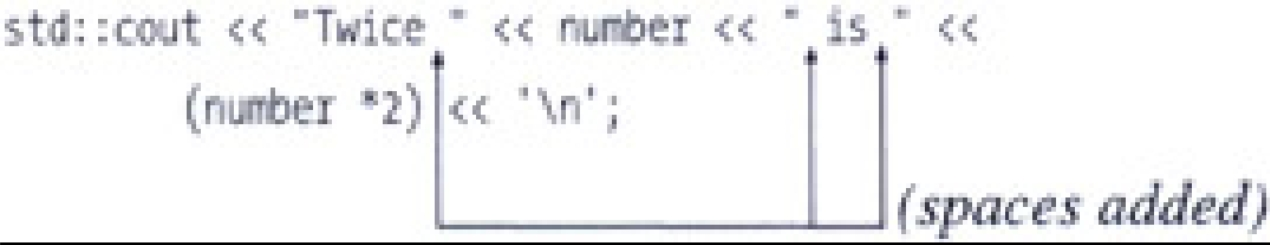
\includegraphics[keepaspectratio,width=0.4\textwidth,height=0.4\textheight]{images/image01.jpg}
\end{flushleft}
